	\begin{center}
            		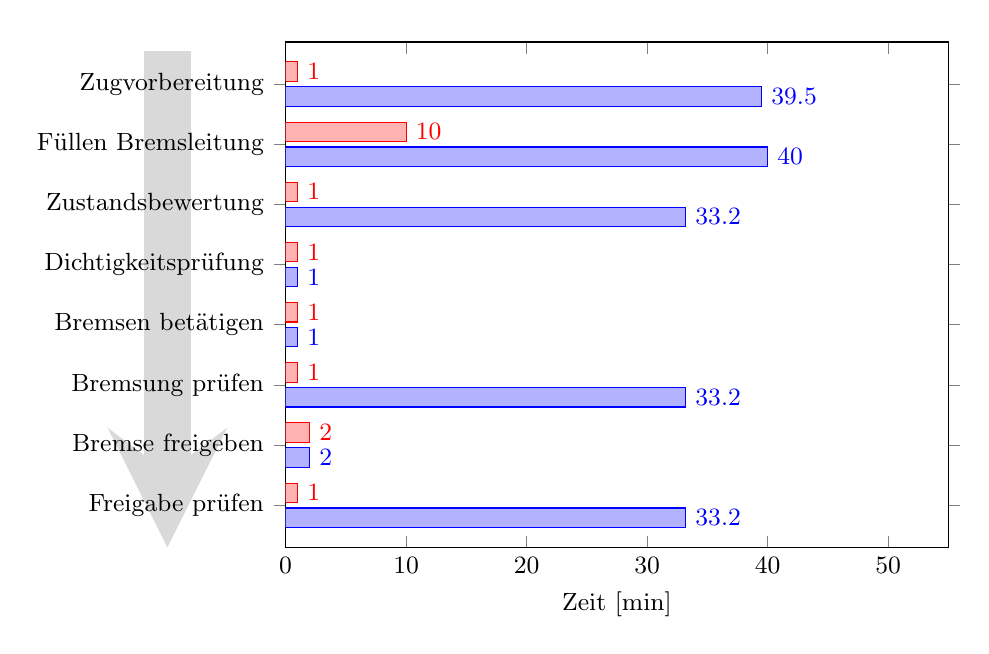
\begin{tikzpicture}[scale = 1]
		\draw[line width = .6cm, gray!30, -stealth] (-1.5,6.3) -- (-1.5,0);
                                \begin{axis}[ 
                                font = \small,
                                width = 10cm, height = 8cm,
                                xbar, xmin=0, xmax = 55,
                                xlabel={Zeit [min]},
                                symbolic y coords={%
                                {Freigabe prüfen},{Bremse freigeben},{Bremsung prüfen}, {Bremsen betätigen}, {Dichtigkeitsprüfung}, {Zustandsbewertung},{Füllen Bremsleitung},{Zugvorbereitung} },
                                ytick=data,
                                nodes near coords, 
                                %nodes near coords align={horizontal},
                                ytick=data,
                                % nodes near coords align={vertical},
                                bar width=7pt,
                %            legend style={
                   %             at={(1,1.1)},
                    %      	anchor=east},
                  %              legend columns = 2,
                                ]
                                \addplot coordinates {                          
                                (39.5,{Zugvorbereitung})
                                (40,{Füllen Bremsleitung})
                                (33.2,{Zustandsbewertung})
                                (1,{Dichtigkeitsprüfung})
                                (1,{Bremsen betätigen})
                                (33.2,{Bremsung prüfen})
                                (2,{Bremse freigeben})
                                (33.2,{Freigabe prüfen})
%                                (183.1,{Sum})
                                };
                                %\addlegendentry{Wagon $<$ 4.0}
                                \addplot coordinates {                          
                                (1,{Zugvorbereitung})
                                (10,{Füllen Bremsleitung})
                                (1,{Zustandsbewertung})
                                (1,{Dichtigkeitsprüfung})
                                (1,{Bremsen betätigen})
                                (1,{Bremsung prüfen})
                                (2,{Bremse freigeben})
                                (1,{Freigabe prüfen})
%                                (18,Sum)
                                };
                                %\addlegendentry{Wagon 4.0}
                                \end{axis}
                              \end{tikzpicture}
        		\end{center}